\documentclass[twoside]{book}

% Packages required by doxygen
\usepackage{fixltx2e}
\usepackage{calc}
\usepackage{doxygen}
\usepackage[export]{adjustbox} % also loads graphicx
\usepackage{graphicx}
\usepackage[utf8]{inputenc}
\usepackage{makeidx}
\usepackage{multicol}
\usepackage{multirow}
\PassOptionsToPackage{warn}{textcomp}
\usepackage{textcomp}
\usepackage[nointegrals]{wasysym}
\usepackage[table]{xcolor}

% NLS support packages
\usepackage[spanish]{babel}
% Font selection
\usepackage[T1]{fontenc}
\usepackage[scaled=.90]{helvet}
\usepackage{courier}
\usepackage{amssymb}
\usepackage{sectsty}
\renewcommand{\familydefault}{\sfdefault}
\allsectionsfont{%
  \fontseries{bc}\selectfont%
  \color{darkgray}%
}
\renewcommand{\DoxyLabelFont}{%
  \fontseries{bc}\selectfont%
  \color{darkgray}%
}
\newcommand{\+}{\discretionary{\mbox{\scriptsize$\hookleftarrow$}}{}{}}

% Page & text layout
\usepackage{geometry}
\geometry{%
  a4paper,%
  top=2.5cm,%
  bottom=2.5cm,%
  left=2.5cm,%
  right=2.5cm%
}
\tolerance=750
\hfuzz=15pt
\hbadness=750
\setlength{\emergencystretch}{15pt}
\setlength{\parindent}{0cm}
\setlength{\parskip}{3ex plus 2ex minus 2ex}
\makeatletter
\renewcommand{\paragraph}{%
  \@startsection{paragraph}{4}{0ex}{-1.0ex}{1.0ex}{%
    \normalfont\normalsize\bfseries\SS@parafont%
  }%
}
\renewcommand{\subparagraph}{%
  \@startsection{subparagraph}{5}{0ex}{-1.0ex}{1.0ex}{%
    \normalfont\normalsize\bfseries\SS@subparafont%
  }%
}
\makeatother

% Headers & footers
\usepackage{fancyhdr}
\pagestyle{fancyplain}
\fancyhead[LE]{\fancyplain{}{\bfseries\thepage}}
\fancyhead[CE]{\fancyplain{}{}}
\fancyhead[RE]{\fancyplain{}{\bfseries\leftmark}}
\fancyhead[LO]{\fancyplain{}{\bfseries\rightmark}}
\fancyhead[CO]{\fancyplain{}{}}
\fancyhead[RO]{\fancyplain{}{\bfseries\thepage}}
\fancyfoot[LE]{\fancyplain{}{}}
\fancyfoot[CE]{\fancyplain{}{}}
\fancyfoot[RE]{\fancyplain{}{\bfseries\scriptsize Generado por Doxygen }}
\fancyfoot[LO]{\fancyplain{}{\bfseries\scriptsize Generado por Doxygen }}
\fancyfoot[CO]{\fancyplain{}{}}
\fancyfoot[RO]{\fancyplain{}{}}
\renewcommand{\footrulewidth}{0.4pt}
\renewcommand{\chaptermark}[1]{%
  \markboth{#1}{}%
}
\renewcommand{\sectionmark}[1]{%
  \markright{\thesection\ #1}%
}

% Indices & bibliography
\usepackage{natbib}
\usepackage[titles]{tocloft}
\setcounter{tocdepth}{3}
\setcounter{secnumdepth}{5}
\makeindex

% Hyperlinks (required, but should be loaded last)
\usepackage{ifpdf}
\ifpdf
  \usepackage[pdftex,pagebackref=true]{hyperref}
\else
  \usepackage[ps2pdf,pagebackref=true]{hyperref}
\fi
\hypersetup{%
  colorlinks=true,%
  linkcolor=blue,%
  citecolor=blue,%
  unicode%
}

% Custom commands
\newcommand{\clearemptydoublepage}{%
  \newpage{\pagestyle{empty}\cleardoublepage}%
}

\usepackage{caption}
\captionsetup{labelsep=space,justification=centering,font={bf},singlelinecheck=off,skip=4pt,position=top}

%===== C O N T E N T S =====

\begin{document}

% Titlepage & ToC
\hypersetup{pageanchor=false,
             bookmarksnumbered=true,
             pdfencoding=unicode
            }
\pagenumbering{alph}
\begin{titlepage}
\vspace*{7cm}
\begin{center}%
{\Large Cifrado Transposicion }\\
\vspace*{1cm}
{\large Generado por Doxygen 1.8.13}\\
\end{center}
\end{titlepage}
\clearemptydoublepage
\pagenumbering{roman}
\tableofcontents
\clearemptydoublepage
\pagenumbering{arabic}
\hypersetup{pageanchor=true}

%--- Begin generated contents ---
\chapter{Indice de namespaces}
\section{Paquetes}
Aquí van los paquetes con una breve descripción (si etá disponible)\+:\begin{DoxyCompactList}
\item\contentsline{section}{\hyperlink{namespace_cifrado_por_transposicion}{Cifrado\+Por\+Transposicion} }{\pageref{namespace_cifrado_por_transposicion}}{}
\end{DoxyCompactList}

\chapter{Indice jerárquico}
\section{Jerarquía de la clase}
Esta lista de herencias esta ordenada aproximadamente por orden alfabético\+:\begin{DoxyCompactList}
\item Form\begin{DoxyCompactList}
\item \contentsline{section}{Cifrado\+Por\+Transposicion.\+Cifrado\+Transposicion}{\pageref{class_cifrado_por_transposicion_1_1_cifrado_transposicion}}{}
\end{DoxyCompactList}
\end{DoxyCompactList}

\chapter{Índice de clases}
\section{Lista de clases}
Lista de las clases, estructuras, uniones e interfaces con una breve descripción\+:\begin{DoxyCompactList}
\item\contentsline{section}{\hyperlink{interface_cifrado_1_1_interface_cifrado}{Cifrado.\+Interface\+Cifrado} }{\pageref{interface_cifrado_1_1_interface_cifrado}}{}
\item\contentsline{section}{\hyperlink{class_cifrado_1_1_transposicion}{Cifrado.\+Transposicion} \\*clase qeu hereda la interfaz \hyperlink{interface_cifrado_1_1_interface_cifrado}{Interface\+Cifrado} que contiene el funcionmiento basico de un metodo de cifrado }{\pageref{class_cifrado_1_1_transposicion}}{}
\end{DoxyCompactList}

\chapter{Documentación de namespaces}
\hypertarget{namespace_cifrado_por_transposicion}{}\section{Referencia del Namespace Cifrado\+Por\+Transposicion}
\label{namespace_cifrado_por_transposicion}\index{Cifrado\+Por\+Transposicion@{Cifrado\+Por\+Transposicion}}
\subsection*{Clases}
\begin{DoxyCompactItemize}
\item 
class \hyperlink{class_cifrado_por_transposicion_1_1_cifrado_transposicion}{Cifrado\+Transposicion}
\begin{DoxyCompactList}\small\item\em fomulario que permite cifrar datos por el metodo de transposicion \end{DoxyCompactList}\item 
class {\bfseries Program}
\end{DoxyCompactItemize}

\chapter{Documentación de las clases}
\hypertarget{class_cifrado_por_transposicion_1_1_cifrado_transposicion}{}\section{Referencia de la Clase Cifrado\+Por\+Transposicion.\+Cifrado\+Transposicion}
\label{class_cifrado_por_transposicion_1_1_cifrado_transposicion}\index{Cifrado\+Por\+Transposicion.\+Cifrado\+Transposicion@{Cifrado\+Por\+Transposicion.\+Cifrado\+Transposicion}}


fomulario que permite cifrar datos por el metodo de transposicion  


Diagrama de herencias de Cifrado\+Por\+Transposicion.\+Cifrado\+Transposicion\begin{figure}[H]
\begin{center}
\leavevmode
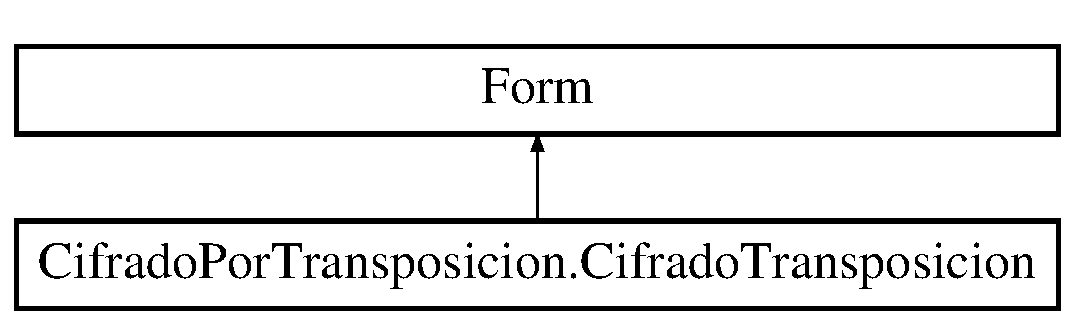
\includegraphics[height=2.000000cm]{class_cifrado_por_transposicion_1_1_cifrado_transposicion}
\end{center}
\end{figure}
\subsection*{Métodos públicos}
\begin{DoxyCompactItemize}
\item 
\hyperlink{class_cifrado_por_transposicion_1_1_cifrado_transposicion_a7b54f34e20c0a9a1c2fc23223ba6d250}{Cifrado\+Transposicion} ()
\begin{DoxyCompactList}\small\item\em Inicializacion del formulario \end{DoxyCompactList}\end{DoxyCompactItemize}
\subsection*{Métodos protegidos}
\begin{DoxyCompactItemize}
\item 
override void \hyperlink{class_cifrado_por_transposicion_1_1_cifrado_transposicion_a7072f986d36a15c6fcc7ccfc0f86f3ec}{Dispose} (bool disposing)
\begin{DoxyCompactList}\small\item\em Limpiar los recursos que se estén usando. \end{DoxyCompactList}\end{DoxyCompactItemize}


\subsection{Descripción detallada}
fomulario que permite cifrar datos por el metodo de transposicion 



\subsection{Documentación del constructor y destructor}
\mbox{\Hypertarget{class_cifrado_por_transposicion_1_1_cifrado_transposicion_a7b54f34e20c0a9a1c2fc23223ba6d250}\label{class_cifrado_por_transposicion_1_1_cifrado_transposicion_a7b54f34e20c0a9a1c2fc23223ba6d250}} 
\index{Cifrado\+Por\+Transposicion\+::\+Cifrado\+Transposicion@{Cifrado\+Por\+Transposicion\+::\+Cifrado\+Transposicion}!Cifrado\+Transposicion@{Cifrado\+Transposicion}}
\index{Cifrado\+Transposicion@{Cifrado\+Transposicion}!Cifrado\+Por\+Transposicion\+::\+Cifrado\+Transposicion@{Cifrado\+Por\+Transposicion\+::\+Cifrado\+Transposicion}}
\subsubsection{\texorpdfstring{Cifrado\+Transposicion()}{CifradoTransposicion()}}
{\footnotesize\ttfamily Cifrado\+Por\+Transposicion.\+Cifrado\+Transposicion.\+Cifrado\+Transposicion (\begin{DoxyParamCaption}{ }\end{DoxyParamCaption})}



Inicializacion del formulario 



\subsection{Documentación de las funciones miembro}
\mbox{\Hypertarget{class_cifrado_por_transposicion_1_1_cifrado_transposicion_a7072f986d36a15c6fcc7ccfc0f86f3ec}\label{class_cifrado_por_transposicion_1_1_cifrado_transposicion_a7072f986d36a15c6fcc7ccfc0f86f3ec}} 
\index{Cifrado\+Por\+Transposicion\+::\+Cifrado\+Transposicion@{Cifrado\+Por\+Transposicion\+::\+Cifrado\+Transposicion}!Dispose@{Dispose}}
\index{Dispose@{Dispose}!Cifrado\+Por\+Transposicion\+::\+Cifrado\+Transposicion@{Cifrado\+Por\+Transposicion\+::\+Cifrado\+Transposicion}}
\subsubsection{\texorpdfstring{Dispose()}{Dispose()}}
{\footnotesize\ttfamily override void Cifrado\+Por\+Transposicion.\+Cifrado\+Transposicion.\+Dispose (\begin{DoxyParamCaption}\item[{bool}]{disposing }\end{DoxyParamCaption})\hspace{0.3cm}{\ttfamily [protected]}}



Limpiar los recursos que se estén usando. 


\begin{DoxyParams}{Parámetros}
{\em disposing} & true si los recursos administrados se deben desechar; false en caso contrario.\\
\hline
\end{DoxyParams}


La documentación para esta clase fue generada a partir de los siguientes ficheros\+:\begin{DoxyCompactItemize}
\item 
C\+:/\+Users/jaira/\+Documents/\+Visual Studio 2015/\+Projects/\+Cifrado\+Por\+Transposicion/\+Cifrado\+Por\+Transposicion/Cifrado\+Transposicion.\+cs\item 
C\+:/\+Users/jaira/\+Documents/\+Visual Studio 2015/\+Projects/\+Cifrado\+Por\+Transposicion/\+Cifrado\+Por\+Transposicion/Cifrado\+Transposicion.\+Designer.\+cs\end{DoxyCompactItemize}

%--- End generated contents ---

% Index
\backmatter
\newpage
\phantomsection
\clearemptydoublepage
\addcontentsline{toc}{chapter}{Índice}
\printindex

\end{document}
